
\documentclass{beamer}
\usepackage{graphicx}
\usepackage[super]{nth}
\usetheme{Malmoe}
\newcommand{\ts}{\textsuperscript}

\makeatletter
    \newenvironment{withoutheadline}{
        \setbeamertemplate{headline}[default]
        \def\beamer@entrycode{\vspace*{-\headheight}}
    }{}
\makeatother

\addtobeamertemplate{navigation symbols}{}{%
    \usebeamerfont{footline}%
    \usebeamercolor[fg]{footline}%
    \hspace{1em}%
    \insertframenumber/\inserttotalframenumber
}

%%%%%%%%%%FIRST SLIDE%%%%%%%%%%

\setbeamercolor*{title}{use=structure,fg=white,bg=structure.fg}
\setbeamertemplate{title page}[default][colsep=-4bp,rounded=true,shadow=true]
\title[Collision Prevention in Distributed 6TiSCH Networks]{Collision Prevention \\in Distributed 6TiSCH Networks}

\author{ Ali Jawad Fahs\\}


\institute[Universities of Somewhere and Elsewhere] % (optional, but mostly needed)
{Universit\'e Grenoble Alpes (UGA) - UFR IM\textsuperscript{2}AG \\
Universit\'e Libanaise Facult\'e de G\'enie (ULFG) \\
Laboratoire d'Informatique de Grenoble (LIG), Team Drakkar \\
VERIMAG,Synchrone }

\date{PhD Interview, \nth{18} of May,2017}


\subject{Wireless Sensor Networks}
%%%%%%%%%%%%%%%%%%%%%%%% OUTLINE%%%%%%%%%%%%
\AtBeginSubsection[]
{ \begin{withoutheadline}
  \begin{frame}<beamer>{Outline}
    \tableofcontents[currentsection,currentsubsection]
  \end{frame}
  \end{withoutheadline}
}

%%%%%%%%%%%%%%%%%%%% SLIDES %%%%%%%%%%%%%%%%
\begin{document}
\begin{withoutheadline}
\begin{frame}
  \titlepage

\begin{itemize}
\item[]
\begin{center}

\includegraphics[width=0.2\linewidth]{logo_im2ag_h122.jpg} \hskip 1em

\includegraphics[width=0.175\linewidth]{logo-ulfg-port.png}  \hskip 1em

\includegraphics[width=0.21\linewidth]{LIG_test.png}  \hskip 1em

\includegraphics[width=0.22\linewidth]{verimag.jpg}
\end{center}
\end{itemize}


\end{frame}
\end{withoutheadline}

\begin{withoutheadline}
    \begin{frame}{Outline} % and our simple frame
        \tableofcontents
    \end{frame}
\end{withoutheadline}

%%%%%%%%%%%%%%%%%%%%%%%%%%%%%INTRO%%%%%%%%%%
\section{Introduction}

\subsection{General intoduction}
\begin{withoutheadline}
\begin{frame}{General intoduction}{IoT \& Wireless Sensor Networks}
\setbeamercolor{block title}{bg=blue!30,fg=black}
\setbeamercolor{block body}{bg=blue!10,fg=black}
\setbeamertemplate{blocks}[rounded][shadow=false]
  \begin{block}{IoT}
    \begin{itemize}
    \item Historically Network was a connection of high performance expensive Computers.
    \item Nowadays Network is a connection of entities with limited processing capabilities called Things. 
    \item  led us to the idea of {\em Intenet of Things (IoT)}
    \end{itemize}
  \end{block}
  
  
    \begin{block}{Wireless Sensor Networks}
    \begin{itemize}
    \item A source of communication between the IoT node.
    \item Main contributions are : low power, low speed, low cost.
    \item  IEEE802.15.4 the main standard for those Networks
    \end{itemize}
    \end{block}

  
  
\end{frame}
\end{withoutheadline}




\begin{withoutheadline}
\begin{frame}{General intoduction}{IEEE802.15.4}

\setbeamercolor{block title}{bg=blue!30,fg=black}
\setbeamercolor{block body}{bg=blue!10,fg=black}
\setbeamertemplate{blocks}[rounded][shadow=false]


\begin{minipage}[t]{0.48\linewidth}

\begin{block}{IEEE802.15.4}
    \begin{itemize}
    \item It defines the low layers of the network (i.e., PHY and MAC) 
    \item Uses RPL routing protocl to create a DODAG graph between the node.
    \item The communication is one-directional between Rx node (Parent), and Tx node (Child). 
    
    \end{itemize}
    \end{block}
\end{minipage}\hfill
\begin{minipage}[t]{0.48\linewidth}
\centering
\begin{figure}[p]

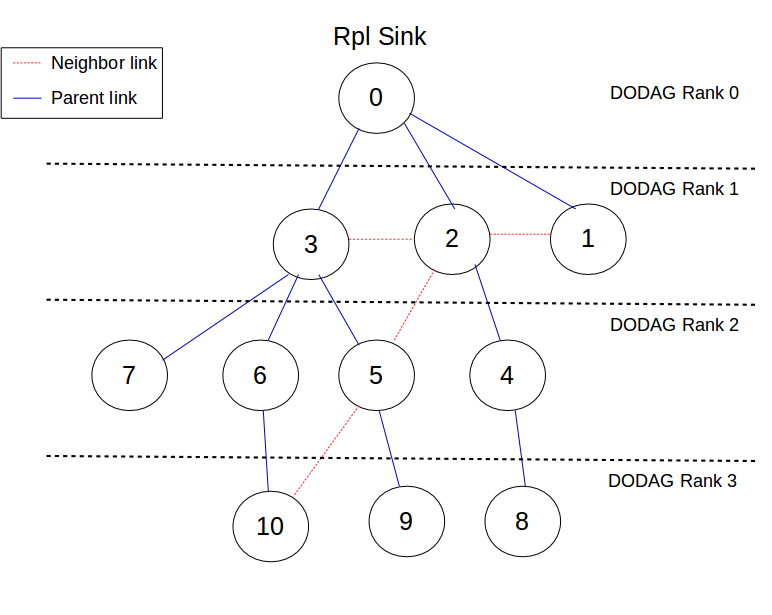
\includegraphics[width=\linewidth]{rpl3.png}
\end{figure}
\end{minipage}

   
    
    

\end{frame}
\end{withoutheadline}




\begin{withoutheadline}
\begin{frame}{General intoduction}{IEEE802.15.4}

\setbeamercolor{block title}{bg=blue!30,fg=black}
\setbeamercolor{block body}{bg=blue!10,fg=black}
\setbeamertemplate{blocks}[rounded][shadow=false]




\begin{block}{IEEE802.15.4e TSCH}
    \begin{itemize}
    \item The Meduim Access Control (MAC) Layer.
    \item Based on Time-slotted Channel Hopping  (TSCH). 
    \item Two types of cells: dedicated and shared.
    \item This table can be managed in centrlized or distributed way. 
    
    \end{itemize}
    \end{block}

\centering
\begin{figure}[p]

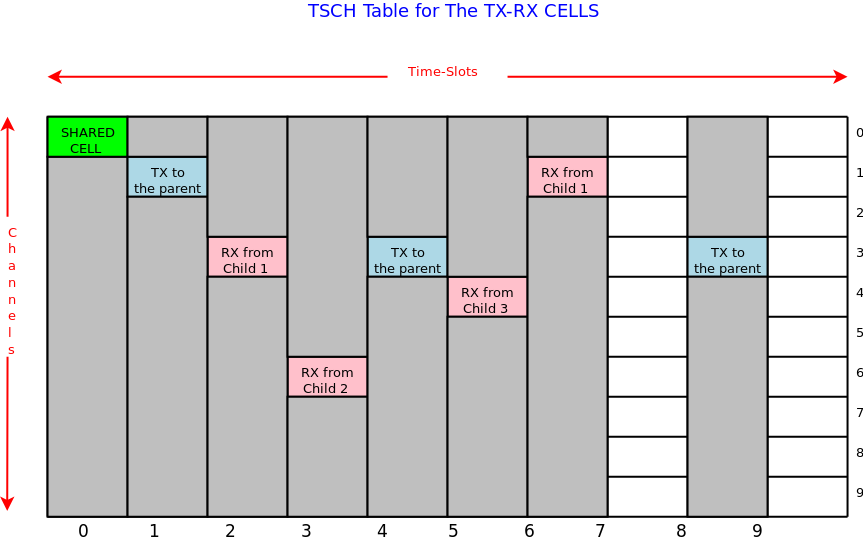
\includegraphics[width=0.6\linewidth]{TSCH.png}
\end{figure}


\end{frame}
\end{withoutheadline}

\begin{withoutheadline}
\begin{frame}{General intoduction}{Collision in the Dedicated Cells}

\setbeamercolor{block title}{bg=blue!30,fg=black}
\setbeamercolor{block body}{bg=blue!10,fg=black}
\setbeamertemplate{blocks}[rounded][shadow=false]

\begin{block}{IEEE802.15.4e TSCH}
    \begin{itemize}
    \item The dedicated cells are supposed to be collision free.
    \item In the distributed approach.Collision occurs in case neighboring nodes select the same TSCH cell.
    \item Collision are very expensive in the Wireless sensor Networks.
      
    \end{itemize}
    \end{block}
  \centering
\begin{figure}[p]

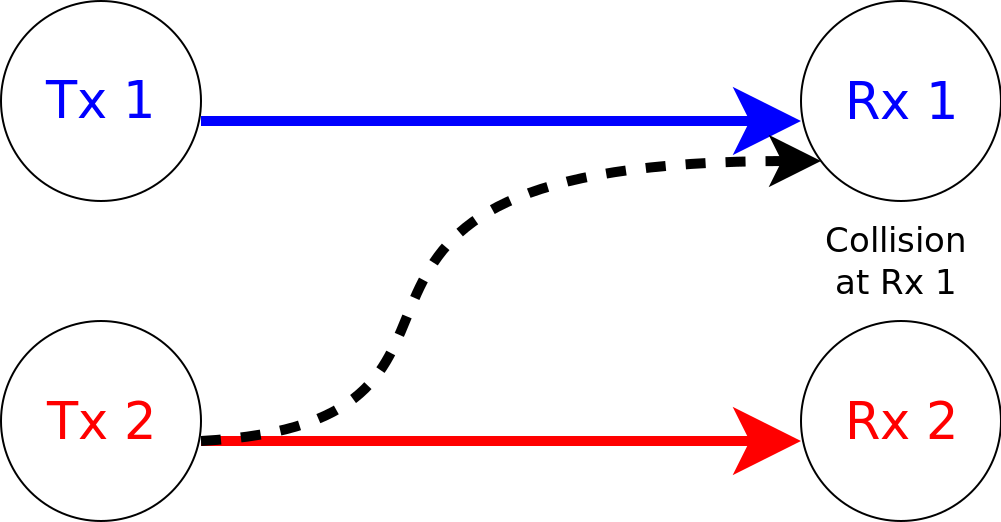
\includegraphics[width=0.6\linewidth]{collision.png}
\end{figure}  
    




\end{frame}
\end{withoutheadline}


\subsection{Project Objectives}
\begin{withoutheadline}
\begin{frame}{Project Objectives}
  \begin{itemize}
  \item {Reducing the collisions in TSCH dedicated cells.}
  \item<2-> {Modifying the Cell reserving process without introducing new overhead on the network}
  \item<3-> {Maintaining a good end-to-end communication latency}

  
  \end{itemize}
\end{frame}
\end{withoutheadline}


%%%%%%%%%%%%%%%%%%%%%%%BACKGROUD%%%%%%%%%%%%%%


\section{Background}
\subsection{IEEE802.15.4e \& 6top}
\begin{withoutheadline}
\begin{frame}{IEEE802.15.4e and 6top}
\setbeamercolor{block title}{bg=blue!30,fg=black}
\setbeamercolor{block body}{bg=blue!10,fg=black}
\setbeamertemplate{blocks}[rounded][shadow=false]




\begin{block}{IEEE802.15.4e \& 6top}
    \begin{itemize}
    \item The standard have defined TSCH schedule but the control of this schedule  was left for other protocols for flexibility and optimization.
    \item 6TiSCH is the merge of IPv6 and TSCH. 
    \item 6TiSCH operation (6top) is a sublayer of 6TiSCH.
    \item 6top is responsible for the cell addition and deletion. 
    
    \end{itemize}
    \end{block}
\end{frame}
\end{withoutheadline}

\begin{withoutheadline}
\begin{frame}{IEEE802.15.4e and 6top}
\setbeamercolor{block title}{bg=blue!30,fg=black}
\setbeamercolor{block body}{bg=blue!10,fg=black}
\setbeamertemplate{blocks}[rounded][shadow=false]


\begin{minipage}[t]{0.48\linewidth}

\begin{block}{6top}

    \begin{itemize}
    \item orchestrates all communications using the TSCH schedule.
    \item allows the nodes to request for new TSCH cells and update the TSCH schedule table accordingly.
    \item 6P enables the distributed scheduling in 6TiSCH network.
    \end{itemize}
    \end{block}

\end{minipage}\hfill
\begin{minipage}[t]{0.48\linewidth}
\centering
\begin{figure}[p]

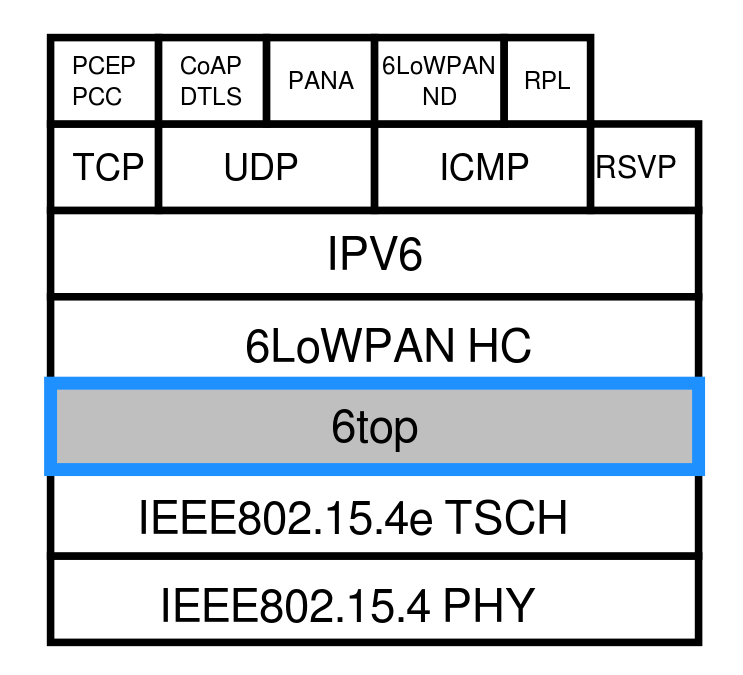
\includegraphics[width=\linewidth]{layers.png}
\end{figure}
\end{minipage}


\end{frame}
\end{withoutheadline}

\begin{withoutheadline}
\begin{frame}{IEEE802.15.4e and 6top}
\setbeamercolor{block title}{bg=blue!30,fg=black}
\setbeamercolor{block body}{bg=blue!10,fg=black}
\setbeamertemplate{blocks}[rounded][shadow=false]




\begin{block}{IEEE802.15.4e \& 6top}
    \begin{itemize}
    \item 6top uses transaction to assign cells to communicating nodes . 
    \item The scheduling function in 6top will choose the cells randomly from TSCH table.
    \item The transaction is done in the shared slot. 
    \item The transaction will be recieved by the neighbor nodes by dropped due too MAC filtering of the messages. 
    
    \end{itemize}
    \end{block}
    \centering
\begin{figure}[p]

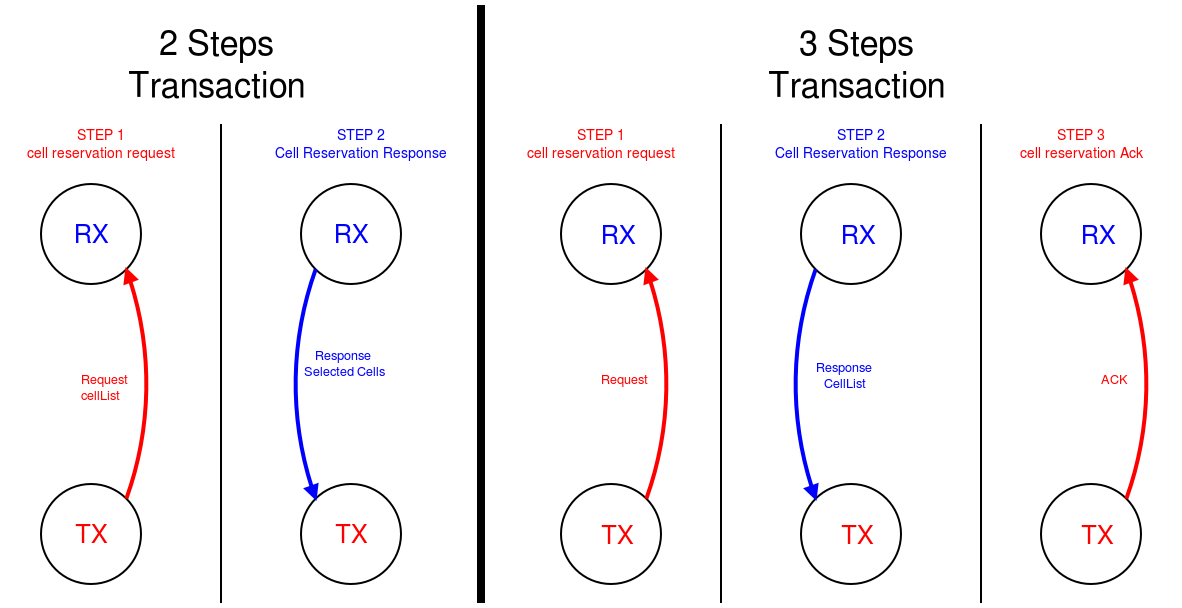
\includegraphics[width=0.7\linewidth]{2,3steps.png}
\end{figure}

\end{frame}
\end{withoutheadline}


\subsection{MAC Filtering}
\begin{withoutheadline}
\begin{frame}{MAC Filtering}
\setbeamercolor{block title}{bg=blue!30,fg=black}
\setbeamercolor{block body}{bg=blue!10,fg=black}
\setbeamertemplate{blocks}[rounded][shadow=false]


  \begin{block}{IEEE802.15.4e \& 6top}
    \begin{itemize}
    \item Consist of level of filters, the first and three levels are related to the correctness of the frame and the mode of the network. 
    \item The fourth level of filters will check the frame destenation and drop it accordingly.
    \item We can Modify the MAC filtering so that we can recieve the frames from 6top. 
    
    
    \end{itemize}
    \end{block}
\end{frame}
\end{withoutheadline}



\subsection{Collisions in Dedicated cells}


  \begin{withoutheadline}
\begin{frame}{6top and Collisions}

\setbeamercolor{block title}{bg=blue!30,fg=black}
\setbeamercolor{block body}{bg=blue!10,fg=black}
\setbeamertemplate{blocks}[rounded][shadow=false]


\begin{block}{6top}

    \begin{itemize}
    \item Nodes have no information about the neighbors.
    \item 6top will select cells randomly form the TSCH schedule. 
    \item If another neighbor node is using the same cell a collision will occur. 
    \item Collisions are expensive.
    \end{itemize}
    \end{block}




\end{frame}
\end{withoutheadline}
%%%%%%%%%%%%%%%%%%%%%%%PROPOSED MECHANISM%%%%%%%%%%%%%%

\section{Proposed Mechanism}

\subsection{Criteria}
\begin{withoutheadline}
\begin{frame}{Proposed Mechanism Criteria}
\begin{itemize}
    \item Our objective is to Reduce the collisions in the dedicatd cells.\pause
    \item Using local mutual execlusion we can prevent collisions.\pause  
    \item Since we are wrking with distributed system, then all the information is local for each node. \pause
    \item Using the 6top transaction we can collect information about neighbors. \pause
    \item From the collected information we can prevent the nodes selecting the same cell. \pause
    \end{itemize}

\end{frame}
\end{withoutheadline}

\subsection{Reserve Table}
\begin{withoutheadline}
\begin{frame}{Reserve Table}


\setbeamercolor{block title}{bg=blue!30,fg=black}
\setbeamercolor{block body}{bg=blue!10,fg=black}
\setbeamertemplate{blocks}[rounded][shadow=false]


\begin{block}

    \begin{itemize}
    \item The nodes will recieve the 6top transaction from the neighbor nodes.
    \item The cells reserved by neighbors will be reserved by a structure similar to TSCH table. 
    \item Scheduling function will avoid selecting cells found in this structure. 
    \item 6top will control this table so any scheduling function can be used with our implementation.
    \end{itemize}
    \end{block}

\centering
\begin{itemize}
\item[]
\begin{center}
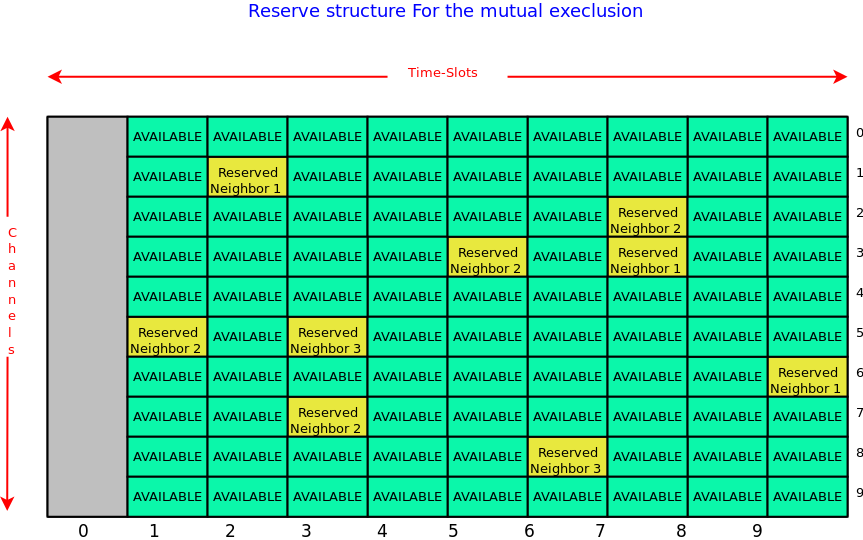
\includegraphics[width=0.5\linewidth]{reserve.png}
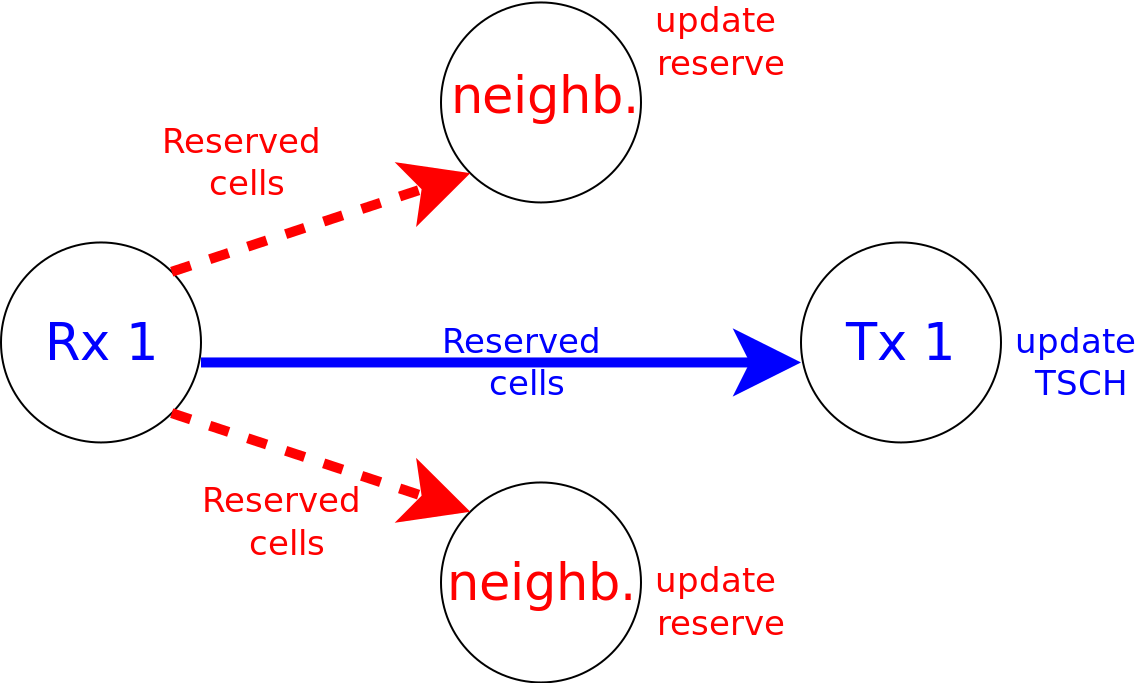
\includegraphics[width=0.5\linewidth]{reserv1.png}
\end{center}
\end{itemize}




\end{frame}
\end{withoutheadline}

\subsection{Adding the Cell Buffer}

\begin{withoutheadline}
\begin{frame}{Cell Buffer}


\setbeamercolor{block title}{bg=blue!30,fg=black}
\setbeamercolor{block body}{bg=blue!10,fg=black}
\setbeamertemplate{blocks}[rounded][shadow=false]


\begin{block}

    \begin{itemize}
    \item The assumption of 100\% successful dilevery is not realistic.
    \item The 6top Transaction maybe lost due too environment effects. 
    \item The loss of the transaction increase the probability of collisions. 
    \item By saving the reserved cells in a buffer, and sending the history of reserved cells this probability can be reduced.
     
    
    \end{itemize}
    \end{block}

\centering
\begin{figure}[p]

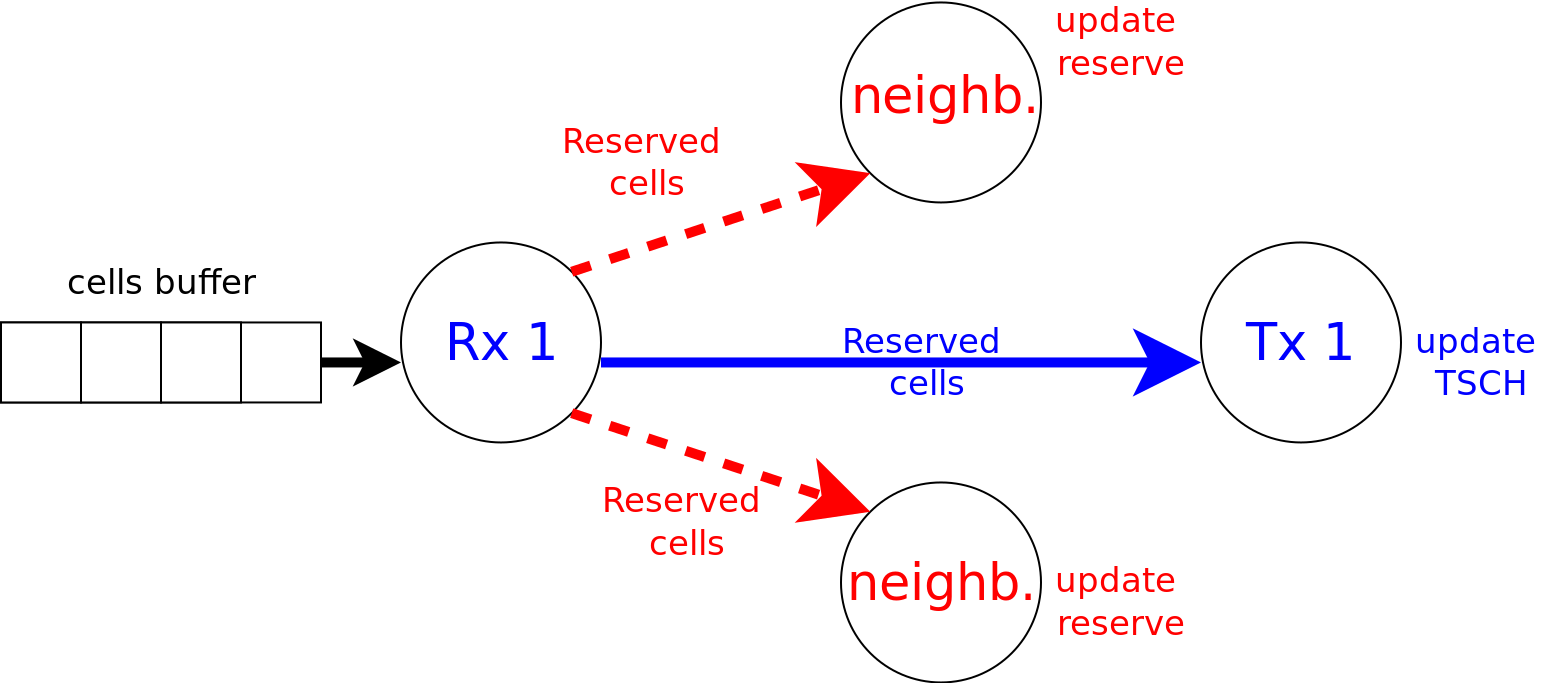
\includegraphics[width=0.7\linewidth]{reserve2.png}
\end{figure}

\end{frame}
\end{withoutheadline}


\begin{withoutheadline}
\begin{frame}{Cell Buffer}

\begin{itemize}
    \item We have created a probablistic model to calaculate the optimal length of the buffer.
    \item $p$ is the probability of successful transmission.
    \item we are confidence with a probability $P_{o}$ that one of the transmission is successful.
    \item $k$ is the number of retransmission (the optimal length of the buffer). 
    \item we end up with the following equation using binomial distribution:
    
    \end{itemize}
    
 \centering
\begin{figure}[p]

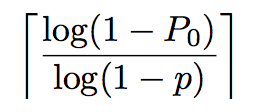
\includegraphics[width=0.3\linewidth]{9nq6n.png}
\end{figure}
\begin{itemize}
\item According to this equation, and by taking the worst case scenario a buffer of length 10 can assure us 95\% of success
 \end{itemize}
\end{frame}
\end{withoutheadline}
%%%%%%%%%%%%%%%%%%%%%%%RESULTS%%%%%%%%%%%%%%

\section{Results}
\subsection{Mechanisim and Results}
\begin{withoutheadline}
\begin{frame}{Mechanisim and Results}


\setbeamercolor{block title}{bg=blue!30,fg=black}
\setbeamercolor{block body}{bg=blue!10,fg=black}
\setbeamertemplate{blocks}[rounded][shadow=false]


\begin{block}{Methodology}

    \begin{itemize}
    \item We used the 6TiSCH simulator \href{https://bitbucket.org/6tisch/simulator/src}{\beamergotobutton{Link}}, the work of watteyne et al. After implementing our approach and fixing some problems in the simultor to make it more realistic. 
    \item Simulations over 100 nodes, over 100 run on the same topology to assure fairness.
    \item We have tried different types of topologies, and had the same results for all of them. 
    \item The simulator updates are in my \href{https://github.com/alijawadfahs/6tisch}{\beamergotobutton{GitHub}}, Results and documentation are in my \href{https://masterthesis2017.000webhostapp.com/}{\beamergotobutton{WIKI PAGE}} along with my reports and daily progress.
    
    \end{itemize}
    \end{block}


\end{frame}
\end{withoutheadline}

\begin{withoutheadline}
\begin{frame}{Results}

\begin{figure}[p]

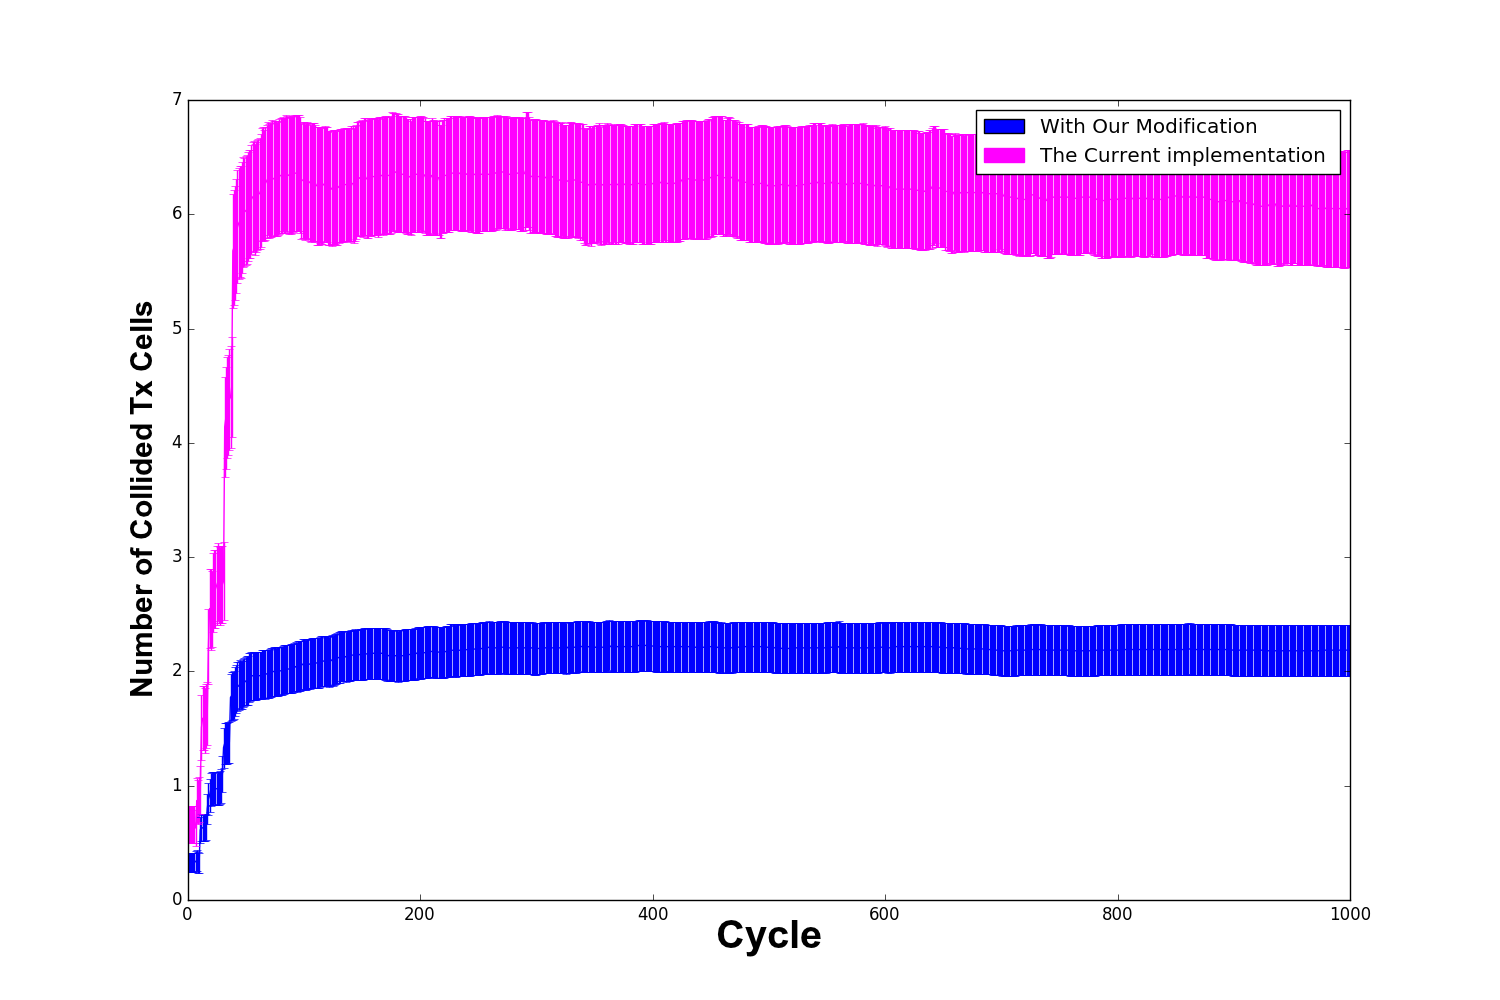
\includegraphics[width=0.95\linewidth]{oie_AlevPnyh9eiC.png}
\caption{Simulation of the Number of Collided Txs Cells as Function of Cycle Number (Time)}
\end{figure}



\end{frame}
\end{withoutheadline}



\begin{withoutheadline}
\begin{frame}{ Results}

\begin{figure}[p]

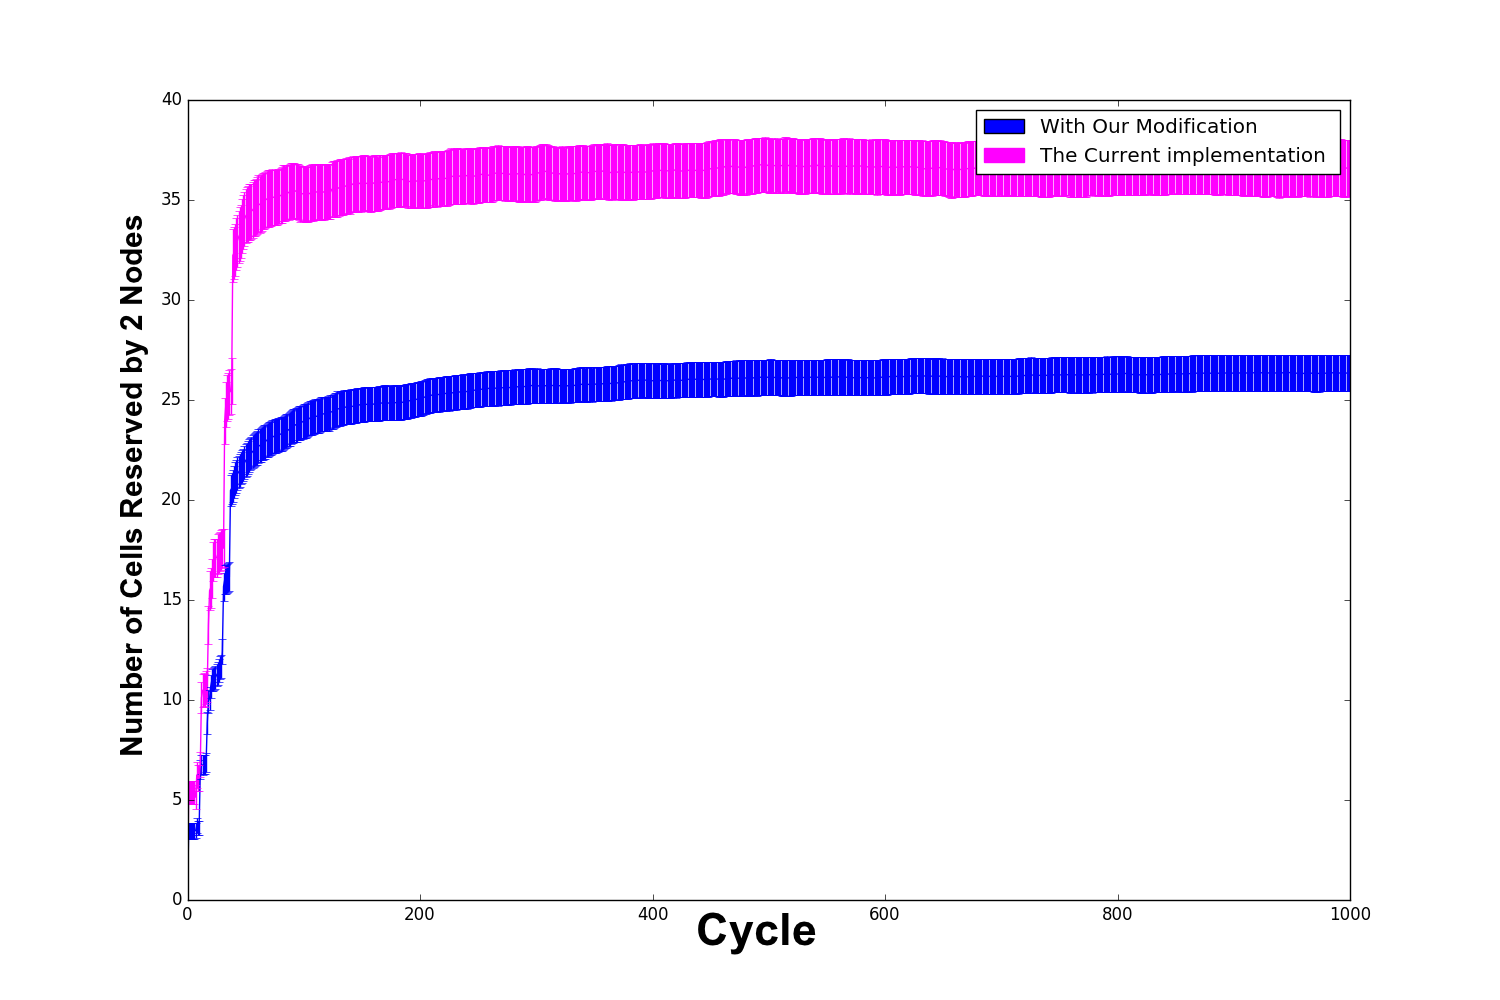
\includegraphics[width=0.95\linewidth]{oie_HDUVTapLLM19.png}
\caption{Simulation of the Number of Cells Reserved by 2 Nodes as Function of Cycle Number (Time)}
\end{figure}



\end{frame}
\end{withoutheadline}

\begin{withoutheadline}
\begin{frame}{Related Work Results comparison}

\begin{figure}[p]

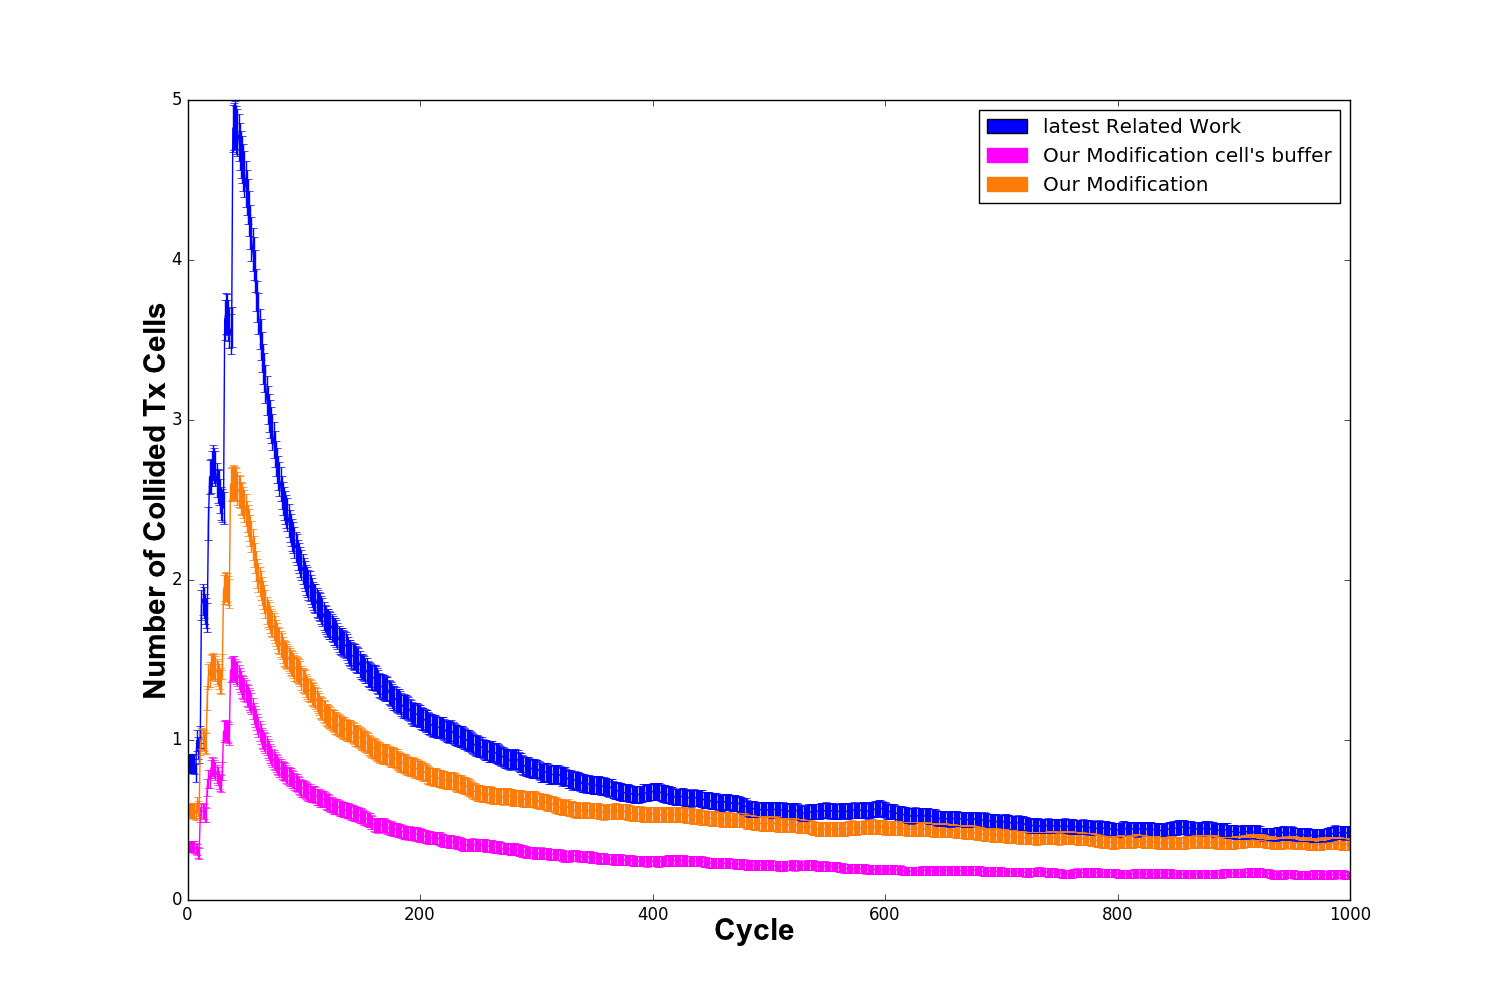
\includegraphics[width=0.95\linewidth]{oie_tsvdkqnj4zdz.png}
\caption{Simulation of the Number of Collided Txs Cells as Function of Cycle Number (Time) - comparison with the housekeeping approach }
\end{figure}



\end{frame}
\end{withoutheadline}

%%%%%%%%%%%%%%%%%%%%%%%SUMMARY%%%%%%%%%%%%%%
\section*{Summary}
\begin{withoutheadline}
\begin{frame}{Summary}
  \begin{itemize}
  \item
    Our implementation introduce  \alert{no overhead } in the network.
  \item
    The implementation \alert{achieved 60\% reduction} in the number of collided Tx cells.
  \item
    The implementation have a positive side effect which is \alert{reducing the interference in the network }.
  \end{itemize}
  
  \begin{itemize}
  \item
    Outlook
    \begin{itemize}
    \item
     Our goal is to reach a place were we have collision free network, using more complex method.
    \item
      Our prespective in this project was work on 6top, but our next steps is to work on the scheduling function to elimante collision.
    \end{itemize}
  \end{itemize}
\end{frame}
\end{withoutheadline}


% All of the following is optional and typically not needed. 
\appendix
\section<presentation>*{\appendixname}
\subsection<presentation>*{For Further Reading}
\begin{withoutheadline}
\begin{frame}[allowframebreaks]
  \frametitle<presentation>{For Further Reading}
    
  \begin{thebibliography}{1}

\bibitem{IEEEhowto:kopka}
Q.Wang, and X. Vilajosana, \emph{ 6top Protocol (6P). Internet Engineering Task Force, Tech. Rep. draft-ietf-6tisch-6top-protocol-00 } \hskip 1em plus
0.5em minus 0.4em\relax https://tools.ietf.org/html/draft-ietf-6tisch-6top-protocol-00 , April 2016.

\bibitem{IEEEhowto:kopka}
T. Watteyne et al, \emph{ Using IEEE 802.15.4e Time-Slotted Channel Hopping (TSCH) in the Internet of Things (IoT): Problem Statement } \hskip 1em plus
  0.5em minus 0.4em\relax https://tools.ietf.org/html/rfc7554 , May 2015.

\bibitem{IEEEhowto:kopka}
T. Winter et al, \emph{ RPL: IPv6 Routing Protocol for Low-Power and Lossy Networks } \hskip 1em plus
  0.5em minus 0.4em\relax https://tools.ietf.org/html/rfc6550 , March 2012.

\bibitem{IEEEhowto:kopka}
D. Dujovne et al, \emph{6tisch: deterministic ip-enabled industrial internet(of things)} \hskip 1em plus
  0.5em minus 0.4em\relax IEEE Communications Magazine — Communications Standards Supplement ,December 2014.
  
\bibitem{IEEEhowto:kopka}
J. Tripathi et al, \emph{A Performance Evaluation Study of RPL: Routing Protocol for Low Power and Lossy Networks} \hskip 1em plus
  0.5em minus 0.4em\relax  Information Sciences and Systems (CISS), 44th Annual Conference on (pp. 1-6). IEEE , March 2010.

\bibitem{IEEEhowto:kopka}
F. Theoleyre and G. Papadopoulos, \emph{Experimental Validation of a Distributed Self-Configured 6TiSCH with Traffic Isolation in Low Power Lossy Networks} \hskip 1em plus
  0.5em minus 0.4em\relax  Proceedings of the 19th ACM International Conference on Modeling, Analysis and Simulation of Wireless and Mobile Systems (pp. 102-110). ACM , November 2017.
  
\bibitem{IEEEhowto:kopka}
N. Accettura et al, \emph{A Decentralized Traffic Aware Scheduling in 6TiSCH Networks: Design and Experimental Evaluation} \hskip 1em plus
  0.5em minus 0.4em\relax   IEEE Internet of Things Journal, 2(6), 455-470 , December 2015.
  
\bibitem{IEEEhowto:kopka}
M. R. Palattella et al, \emph{On-the-Fly Bandwidth Reservation for 6TiSCH Wireless Industrial Networks} \hskip 1em plus
  0.5em minus 0.4em\relax  IEEE Sensors Journal, 16(2), 550-560,  September 2015.
  
\bibitem{IEEEhowto:kopka}
M. R. Palattella et al, \emph{Traffic Aware Scheduling Algorithm for Reliable Low-Power Multi-Hop IEEE 802.15.4e Networks} \hskip 1em plus
  0.5em minus 0.4em\relax  IEEE 23rd International Symposium on Personal, Indoor and Mobile Radio Communications - (PIMRC),  September 2012.
 
\bibitem{IEEEhowto:kopka}
N. Accettura et al, \emph{Decentralized Traffic Aware Scheduling for Multi-hop Low Power Lossy Networks in the Internet of Things} \hskip 1em plus
  0.5em minus 0.4em\relax   In World of Wireless, Mobile and Multimedia Networks (WoWMoM), 2013 IEEE 14th International Symposium and Workshops on a (pp. 1-6). IEEE,  June 2013.
 
\bibitem{IEEEhowto:kopka}
S. Duquennoy et al, \emph{Orchestra: Robust Mesh Networks Through Autonomously Scheduled TSCH} \hskip 1em plus
  0.5em minus 0.4em\relax  Proceedings of the 13th ACM Conference on Embedded Networked Sensor Systems (pp. 337-350). ACM, November 2015.

\bibitem{IEEEhowto:kopka}
K. Muraoka et al, \emph{Simple Distributed Scheduling With Collision Detection in TSCH Networks} \hskip 1em plus
  0.5em minus 0.4em\relax  IEEE Sensors Journal, 16(15), 5848-5849,  May 2016.
  
\bibitem{IEEEhowto:kopka}
L. Lamport, \emph{Time, clocks, and the ordering of events in a distributed system} \hskip 1em plus
  0.5em minus 0.4em\relax  Communications of the ACM, 21(7), 558-565, July 1978.
  
\bibitem{IEEEhowto:kopka}
T. P. Duy , \emph{Distributed cell selection for scheduling function in 6TiSCH networks} \hskip 1em plus
0.5em minus 0.4em\relax Computer Standards and Interfaces, 53, 80-88, March 2017.

\end{thebibliography}
\end{frame}
\end{withoutheadline}
\end{document}


